\chapter{\xlabel{dimm}The Dynamic Iterative Map-Maker Explained}
\label{sec:dimm}

The Dynamic Iterative Map-Maker, hereafter just referred to as the
map-maker is the tool you will use to produce SCUBA-2 maps, and is
implemented by the \smurf\ \makemap\ command. It performs
all pre-processing steps to clean the data, followed by solving for
multiple signal components using an iterative algorithm, and binning
the resulting time-series data to produce a final science map.

The \makemap\ command can be invoked in two ways: 1) directly by typing
``\texttt{makemap}'' in response to a unix shell prompt (see
\cref{Section}{sec:manual}{Running \task{makemap} outside the pipeline}), or 2)
indirectly as part of an \oracdr\ recipe (see
\cref{Chapter}{sec:pipe}{The SCUBA-2 Pipeline}).

\textbf{This chapter describes how the map-maker produces a science image
from raw SCUBA-2 data. It should be considered essential reading as it
provides an understanding of how your reduced image was produced. This is
particularly true if you wish to modify the default map-maker parameters.}
\color{red}\textbf{ If you prefer to jump straight in to the data reduction go
to \cref{Chapter}{sec:pipe}{The SCUBA-2 Pipeline}.}\color{black}


\section{\xlabel{dimm_theory}How it works}

The time-varying signal recorded by a bolometer, $b(t)$, contains
contributions from a variety of sources:

\begin{equation}
\label{eq:bolsig}
b(t) = e(t) \times a(t) + n^{\textrm{w}}(t) + gn^{\textrm{c}}(t) + n^{\textrm{f}}(t),
\end{equation}

where $e(t)$ is the atmospheric extinction, $a(t)$ is the astronomical
signal (time varying as the telescope scans across the sky),
$n^{\textrm{w}}(t)$ is the uncorrelated white noise, $g$ is an
optional scalefactor which is unique to each bolometer,
$n^{\textrm{c}}(t)$ is the correlated (or, common mode) signal, and
$n^{\textrm{f}}(t)$ is the (predominantly low-frequency) noise which
does not have a simple correlation relationship that would be included
in the $n^{\textrm{c}}(t)$ noise term.

The map-maker works by producing individual models of the various
components that make up the signal recorded by each bolometer.  It
models and removes the extinction and noise components in order of
decreasing magnitude, ultimately leaving just the astronomical signal
plus residual noise.  The modelled components are listed in
\cref{Table}{tab:mods}{tabulated} and described more fully in
\cref{Section}{sec:models}{The individual models}.

\textbf{A \emph{configuration file} should usually be supplied when
running \makemap\ directly.} This file holds a set of parameter values
that control all aspects of the map-maker, including details of the
pre-processing steps, which model components to include, parameters that
control the determination of each model, and the stopping (or
convergence) criteria. If no configuration file is supplied when running
\makemap\footnote{\emph{i.e.} you include ``\texttt{config=def}'' on the
\makemap\ command line.}, a set of default parameter values will be used.
There are a great number of these parameters, but fortunately not all of
them are of interest to the typical user. \cref{Appendix}{app:parameters}{}
documents the parameters you are more likely to find of interest,
including the default value that is assigned to each parameter if you do
not give it a value in your configuration file.  For a full list of all
available parameters, see the appendix \xref{``Configuration Parameters''}
{sun258}{par_full} within \xref{SUN/258}{sun258}{}.

It is possible to create a map without supplying a configuration file to
\makemap\ (\emph{i.e.} leaving all configuration parameters set to their default
values---``\texttt{config=def}''---when running \texttt{makemap}) but it is not
recommeneded since it will not give optimal results
for your particular observation. For this reason, specialised
configuration files have been developed which are tailored to different
science goals, be they detecting faint galaxies or mapping large
molecular clouds. A description of these specialised configuration files
can be found \cref{in Section}{sec:config}{here}.

\textbf{Note:} When using the pipeline to create a map, rather than running
\makemap\ directly, the pipeline will always use a configuration
file---one of the standard configuration files will be selected if none is
specified by you.

\section{The reduction step-by-step}% (Following \underline{\href{https://ui.adsabs.harvard.edu/abs/2013MNRAS.430.2545C/abstract}{Chapin et al. (2013)}})}
\label{sec:algorithm}

This section describes the basic map-making process used by the
default configuration.  It may be modified in many ways by supplying a
configuration file containing alternative parameter values.

\cref{Figure}{fig:dimm}{The graphic below} shows the flow chart of the
basic map-making process. It is divided into two sections: the pre-processing
stage where the data are cleaned, then the iterative stage where the different
models are subtracted, a sky map created and the convergence checked.


\begin{enumdesc}
\item[Initial cleaning and down-sampling]
  The separate raw data files are first concatenated into a single time
  series for each sub-array (if possible---see \latexhtml{the description
  of \emph{Data Chunking} on Page~\pageref{box:chunk})~}{\htmlref{Data
  Chunking)}{box:chunk}} and have the flat-field from the associated
  fast-flat scans applied to calibrate the bolometers.  This resulting
  time-series are in units of pW.

  These time-series are then re-sampled at a rate that matches the
  requested pixel size---the equivalent to applying a low-pass filter.
  Down-sampling saves time and memory usage when running the map-maker,
  without losing any significant information. The degree of
  down-sampling applied depends on how fast the telescope was moving
  during the observation, the requested pixel size. In general, slower
  scans will be more heavily down-sampled than faster scans, and fast
  scans may not be down-sampled at all.

  A number of cleaning steps are then run: bolometers that have unusually
  high noise levels are identified and excluded from further processing,
  any sudden steps in the base-line of each bolometer are identified and
  corrected, and a polynomial estimate of the base-line is removed from
  each bolometer.

\item[Iterative steps]

  Next comes the iterative stage. In each iteration, estimates are
  produced for each model component. These are removed from the cleaned
  time-series data and the remaining data values are binned into a map.
  However, in general, the presence of astronomical signal within the
  original time series will have upset the estimates of the \model{COM},
  \model{GAI} and \model{FLT} models, causing the final map to be
  inaccurate. But now that we have a map (albeit an inaccurate map), we
  can sample the map at the position of each bolometer value to get an
  estimate of the astronomical component within the original time-series
  data. We then remove this astronomical signal from the original
  time-series data and re-estimate the models. These new model estimates
  should be more accurate since they are not so heavily
  influenced by the astronomical signal. In turn, this allows us to
  create a more accurate map.  We repeat this process until the map does
  not change significantly with further iterations. Whilst not
  mathematically rigorous, we expect the process to converge because the
  astronomical signal is in general much smaller than any of the other
  components and so each iteration introduces a very small fractional
  change in the model estimates.

  Within each iteration, the first components to be modelled and removed
  are \model{COM} and \model{GAI}, which work together to calculate and
  remove the average signal template of all bolometers, allowing each
  bolometer to have an arbitrary gain and offset. In addition, the
  \model{GAI} model will flag as unusable any bolometer in which the
  signal looks very different to the common-mode.

  The next model
  (\model{EXT}) applies a multiplicative extinction correction to the
  data. Following this, the \model{FLT} model filters each bolometer
  time-stream independently to remove low frequencies that correspond
  to angular scales larger than 600\,arcsec and 300\,arcsec at
  450$\mu$m and 850$\mu$m, respectively.

  After these models have been removed, the AST model (\emph{i.e.} the
  estimate of the astronomical signal) produced by the previous iteration,
  is added back onto the remaining time-series data\footnote{This step is
  omitted on the first iteration since no estimate of AST has yet been
  created.}, and the new values are binned up on the sky to produce a new
  estimate of the final science map.  Since many samples typically
  contribute to the estimate of the signal in a given pixel, the noise is
  greatly reduced compared with the time-series data. The variance of
  each map pixel value is determined from the spread of sample values
  that contribute to the pixel.  The value of this map at the position
  of each bolometer sample is then found. This forms the new \model{AST}
  model which is removed from the time-streams, leaving just the residual
  noise.

  The \model{NOI} model then measures the noise in the residual signals
  for each bolometer to establish weights for the data as they are placed
  into the map in subsequent iterations. This is only done on the first
  iteration. Subsequent iterations re-use the weights established on the
  first iteration.

\item[Checking convergence]

  Convergence is checked against the parameters detailed in the
  configuration file. Convergence is achieved either when the requested
  number of iterations has been completed, or when the mean change in the
  map pixel values is less than a specified fraction of a standard
  deviation (see parameter \xparam{MAPTOL}{maptol}).  If more iterations
  are required or (in the latter case) the map is still changing
  significantly, all the model---\emph{except for AST}---are added
  back onto the residuals, thus reconstructing the original time-series
  but without the astronomical signal.  This is the signal upon which the
  model estimates will be based on the next iteration.

\end{enumdesc}


\starfig{sc21_flow_dimm_blue}{}{width=0.78\linewidth}{fig:dimm}{
  Flowchart of the map-maker}{ A flow chart illustrating the dynamic
  iterative map-maker. Note that for each iteration the \model{AST}
  model is subtracted from the time-series leaving only those
  contributions to be fitted and removed.  }

For full details of the map-maker see \textbf{Chapin et al. (2013)}
\cite{mapmaker}.

\setlength{\extrarowheight}{3pt}
\begin{table}
\centering
\begin{tabular}{c|l}
\hline
\textbf{Model} &\hspace{0.2cm} \textbf{Description} \\
\hline
\model{COM}&\hspace{0.2cm} Common-mode signal\\
\model{GAI}&\hspace{0.2cm} Gains that scale each bolometer to the common-mode\\
\model{EXT}&\hspace{0.2cm} Extinction correction\\
\model{FLT}&\hspace{0.2cm} Filter that removes low frequencies\\
\model{AST}&\hspace{0.2cm} Astronomical signal\\
\model{NOI}&\hspace{0.2cm} Residual noise\\
\hline
\end{tabular}
\caption{\small Table adopted from Chapin et al. (2013). A detailed
explanation of each model is given in \cref{Section}{sec:models}{The individual models}.}
\label{tab:mods}
\end{table}

\raggedbottom

\begin{sltextbox}{Data Chunking}
  \renewcommand\figurename{Data Chunking}
  \renewcommand{\thefigure}{}
  \renewcommand{\thefigure}{}
  \caption{}
  \label{box:chunk}
  Chunking occurs when there is insufficient computer memory available
  for the map-maker to process all the time-series data together, or when
  there is a gap in the data (e.g.  from a missing sub-scan). In these
  cases, the map-maker divides up the time-series data into a number of
  ``chunks'' and produces a map from each chunk independently, before
  re-combining all the maps at a later stage to create the final map.
  Ideally you want your data reduced in a single chunk, however this can
  be unfeasible for large maps.

  The more data the map-maker processes at once, the better chance it
  has of determining the difference between sky signal and background
  noise.

  Information about chunking can be obtained in several ways:
  \begin{itemize}

  \item The screen output generated by \makemap\ will include one or more
  statements about chunking, such as:
  \begin{terminalv}
smf_iteratemap: Continuous chunk 1 / 1 =========
  \end{terminalv}
  The final number indicates the number of chunks being used (one in
  this case).

  \item The MEMLOW FITS header in the final map can be examined to
  determine if chunking occurred due to insufficient memory. For
  instance:
  \begin{terminalv}
% fitsval mymap memlow
FALSE
  \end{terminalv}
  indicates that the map in file \texttt{mymap.sdf} did not suffer from
  chunking as a result of low memory.

  \item The NCONTIG FITS header in the final map can be examined to
  determine if chunking occurred due to the supplied input data being
  discontiguous. For instance:
  \begin{terminalv}
% fitsval mymap ncontig
2
  \end{terminalv}
  indicates that the time-series data from which \texttt{mymap.sdf} was
  created was broken into two contiguous groups of samples. This
  indicates a potential problem with the data---the NCONTIG header
  should normally be one.
  \end{itemize}

  In \textsc{daisy} mode chunking is less of a concern as the entire
  map area is covered many times in the space of a single observation.

  For \textsc{pong} maps chunking is a bigger concern, with the
  maximum number of chunks that can be tolerated dependent on the
  number of map rotations. For example, a 40-minute \textsc{pong} map
  with eight rotations may get divided into three or four
  chunks. Although not ideal, this will mean that each point is still
  covered by two or three passes. Fewer passes than this however and
  the map-maker become less effective.

  Be aware that focus observations are intentionally dis-contiguous. If
  you attempt to make a map from a focus observation, it will be
  processed in several chunks no matter how much memory your computer has.
\end{sltextbox}

\section{\xlabel{models}The individual models}
\label{sec:models}

The list of models to be evaluated (and removed) by the map-maker, and
the order in which they are used during the iterative stage, is given by
the \xparam{MODELORDER}{modelorder} parameter in the configuration file.
These models are modular however, so their order may be changed. The
default model order is given below\footnote{If using \textsc{starlink}'s PCA background removal, one can add ``pca'' to the list: (com,gai,pca,ext,flt,ast,noi). For more information, see \href{https://www.eaobservatory.org/jcmt/2019/03/faster-pca/}{https://www.eaobservatory.org/jcmt/2019/03/faster-pca/}}.

\begin{terminalv}
modelorder = (com,gai,ext,flt,ast,noi)
\end{terminalv}

The only configuration file not following this model order is the one tailored
for blank field maps which does not include a \model{FLT} model in the
iterative stage but instead includes an equivalent high-pass filter
as part of the cleaning stage (see \cref{Section}{sec:config}{Specialised
configuration files}).

Below is an introduction to each model. More complete descriptions of the
models and all the associated caveats can be found in Chapin et al.
(2013) \cite{mapmaker}. Details of each model are controlled by a set of
configuration parameters that begin with the name of the model. For
instance, all parameters related to the \model{COM} model will be of the
form ``\param{COM.xxx}''.

\begin{longtable}{c p{0.8\textwidth}}
  \hline
  \textbf{MODEL} & \multicolumn{1}{c}{\textbf{DESCRIPTION}}\\
  \hline
  \endhead
  \ifpdf
  \hline
  \endfoot
\fi
  COM& The \model{COM} model removes the common-mode signal
  (the signal that is common to all bolometers), the dominant
  contributor to this signal being the sky noise. It determines this
  by simply averaging over all bolometers for each time slice.
  Bolometers are flagged as bad, (and thus omitted from the final
  map), if they do not resemble the \model{COM} model seen by the
  majority of the other bolometers.

  Extended emission on a scale larger than the array footprint on the
  sky will contribute a signal indistinguishable from a common-mode
  signal. This puts an upper limit on the spatial scale of
  astronomical emission that can be recovered\footnote{``Fake Sources'' of
  known properties can be inserted into the raw SCUBA-2 time stream
  in order to evaluate the extent of robust emission recovery. For
  more information, see
  \href{https://ui.adsabs.harvard.edu/abs/2015MNRAS.454.2557M/abstract}{Mairs et al. 2015} (\cite{extendedrecovery})}.\\
  \hline
GAI& \model{GAI} model works with \model{COM} in removing the
  common-mode signal. \model{GAI} consists of a time-varying scale
  and offset for each bolometer, which scales the \model{COM} model
  so that it resembles the original bolometer data as closely as possible.
  It is the scaled version of \model{COM} that is removed from the
  bolometer time-series.  In addition, the \model{GAI} model identifies
  any bolometers that looks very different to the common-mode signal, and
  flags them as unusable. \\
\hline
EXT& \model{EXT} applies the extinction correction. This is a
  time-varying scaling factor that is derived from the JCMT
  water-vapour radiometer. As it deals with 30-second chunks of data,
  this accounts for varying conditions over a long observation. For
  more details see \cref{Appendix}{app:cal}{SCUBA-2 data
    calibration}.\\
\hline
FLT& The \model{FLT} model acts on the Fourier transform of the
  bolometer data. High-pass (only allows \textit{higher} frequencies
  to pass) and low-pass (only allows \textit{lower} frequencies to
  pass) filters can be specified. These cut-off frequencies can either
  be specified directly in Hz, or as an angular spatial scale in
  arcseconds that is subsequently converted into a frequency using
  the speed at which the telescope is moving. The most important role of
  this model is to apply a high-pass filter in order to remove the
  low frequency $1/f$ noise. Note that extended emission varies slowly
  over the array; it therefore appears at low frequencies and complicates
  the choice of a high-pass filter. A further discussion of this matter is
  given in \cref{Section}{sec:bright_ex}{Extended galactic sources}.\\
\hline
AST& The \model{AST} model is generated in conjunction with a
  science map. Hence, the position of \model{AST} in the model order
  indicates at what stage the astronomical image should be
  estimated. When the \model{AST} model is calculated, the first step is
  bin the residual time-series data into a map (using nearest-neighbour
  sampling). Following this, the map is projected back into the time
  domain (\emph{i.e.} sampled at the position of every bolometer sample)
  and removed as the \model{AST} model.\\
\hline
NOI& \model{NOI} should come last in the model order and
  calculates the RMS noise level in each bolometer.  It is only
  calculated on the first iteration. The same noise levels are then used
  on all subsequent iterations to weight the bolometer values when
  binning them into a map. Each bolometer may have a single noise estimate
  that remains fixed over the whole observation, or may have multiple
  noise levels, each of which relate to a different part of the observation.
  See parameters \xparam{NOI.BOX_SIZE}{noi.box\_size}
  and \xparam{NOI.BOX_TYPE}{noi.box\_type}. \\
\hline
\end{longtable}

Examples of the time traces for a single bolometer from these
models is shown in \cref{Figure}{fig:itercomp}{time-domain
components}. These traces cover a subset of an observation of the
secondary calibrator CRL~2688. You can clearly see the dominance of the
\model{COM} model which is removed first. The \model{FLT} model
stores the data removed by the high-pass filter. In the \model{AST}
model, CRL~2688 is clearly seen as positive spikes which appear when
the bolometer passes over the source. Finally, the residual signal
stored in \model{RES} is flat, indicating that most of the signal has
been successfully accounted for by the other model components.

\begin{figure}
\begin{center}
  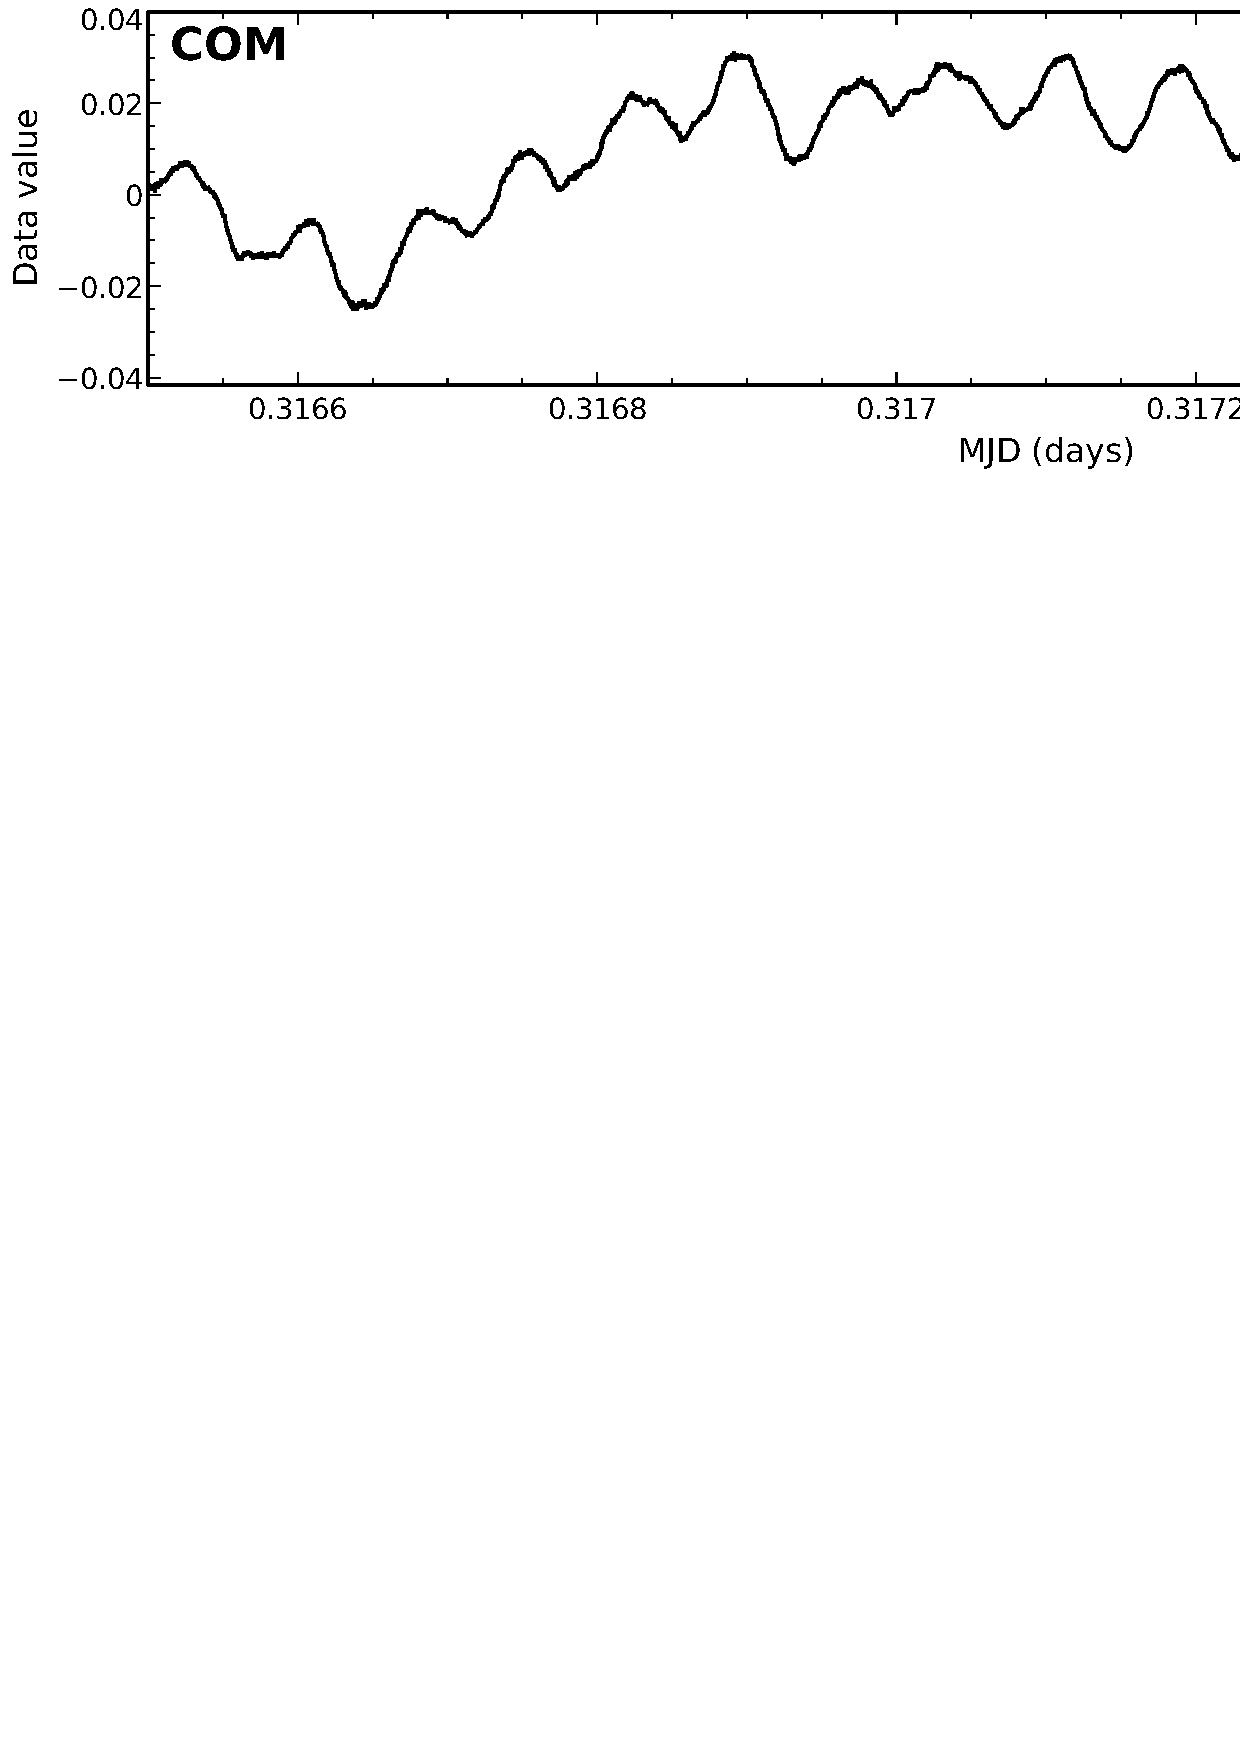
\includegraphics[width=\linewidth]{sc21_com} \\
  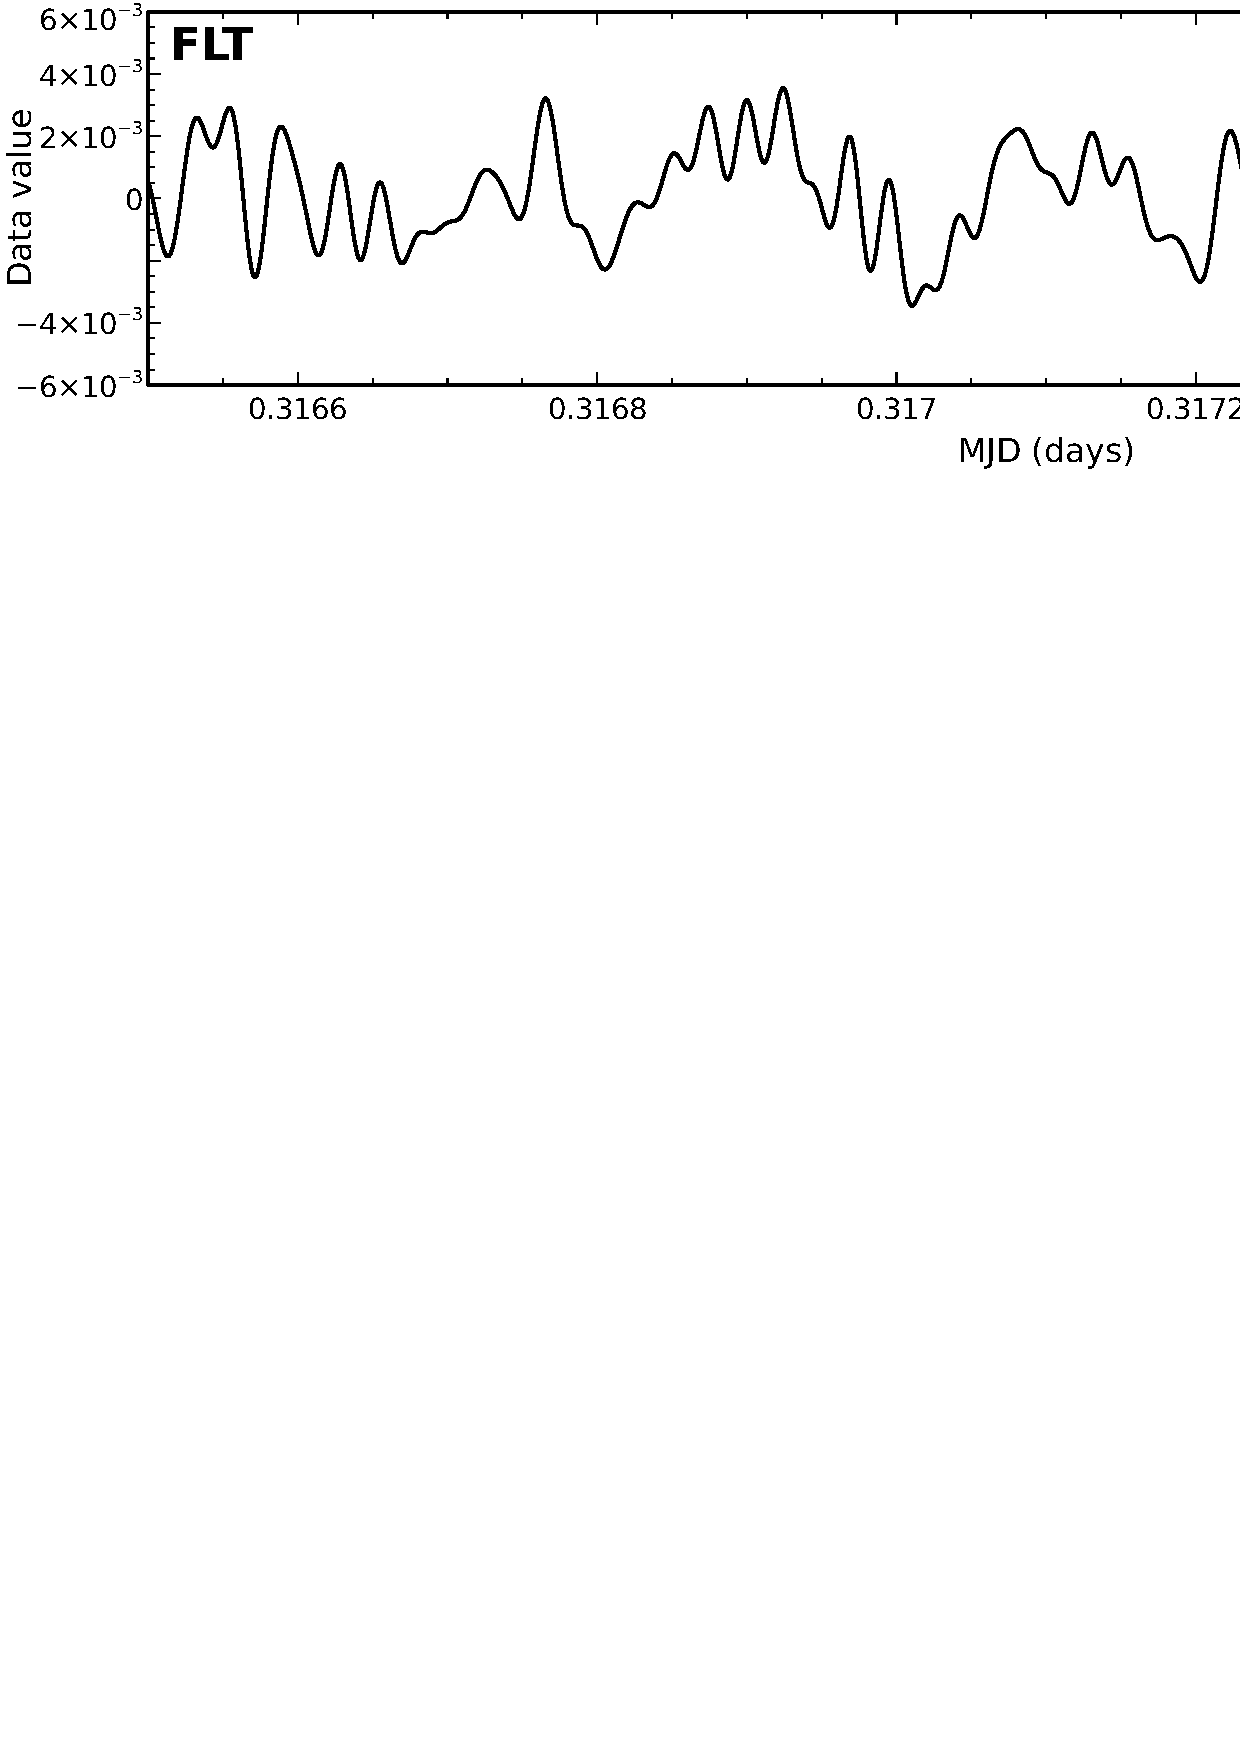
\includegraphics[width=\linewidth]{sc21_flt} \\
  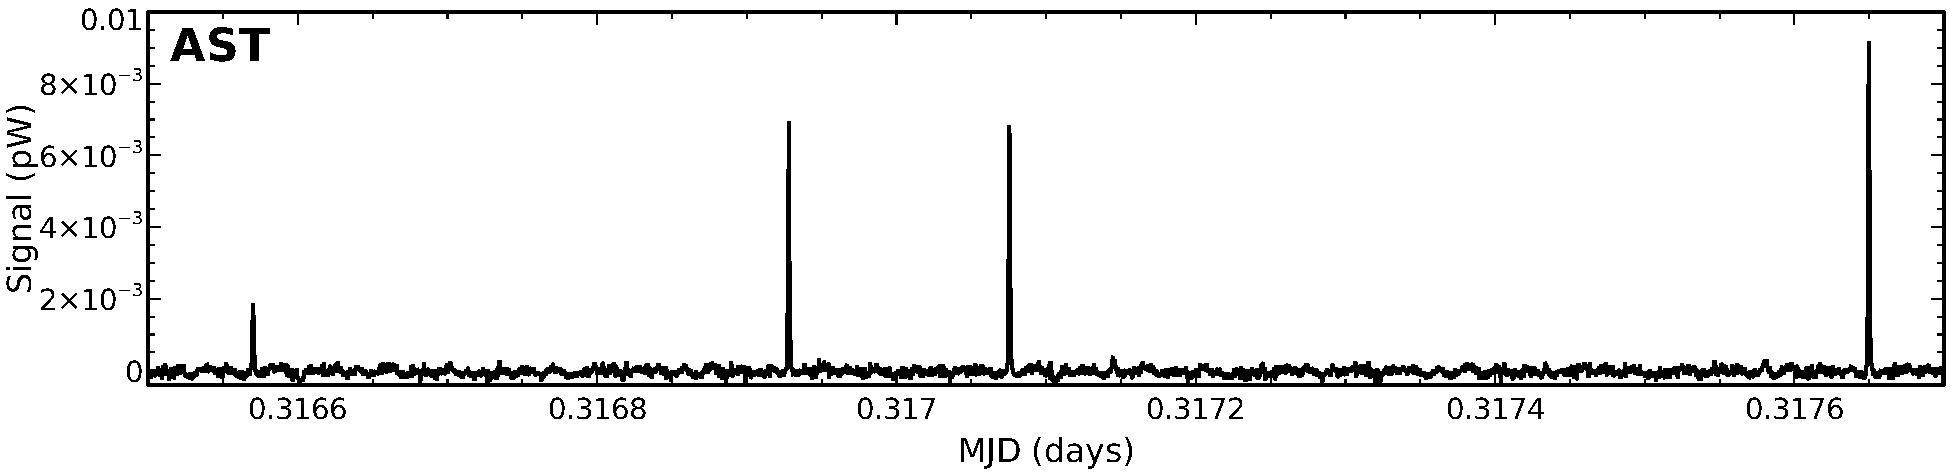
\includegraphics[width=\linewidth]{sc21_ast} \\
  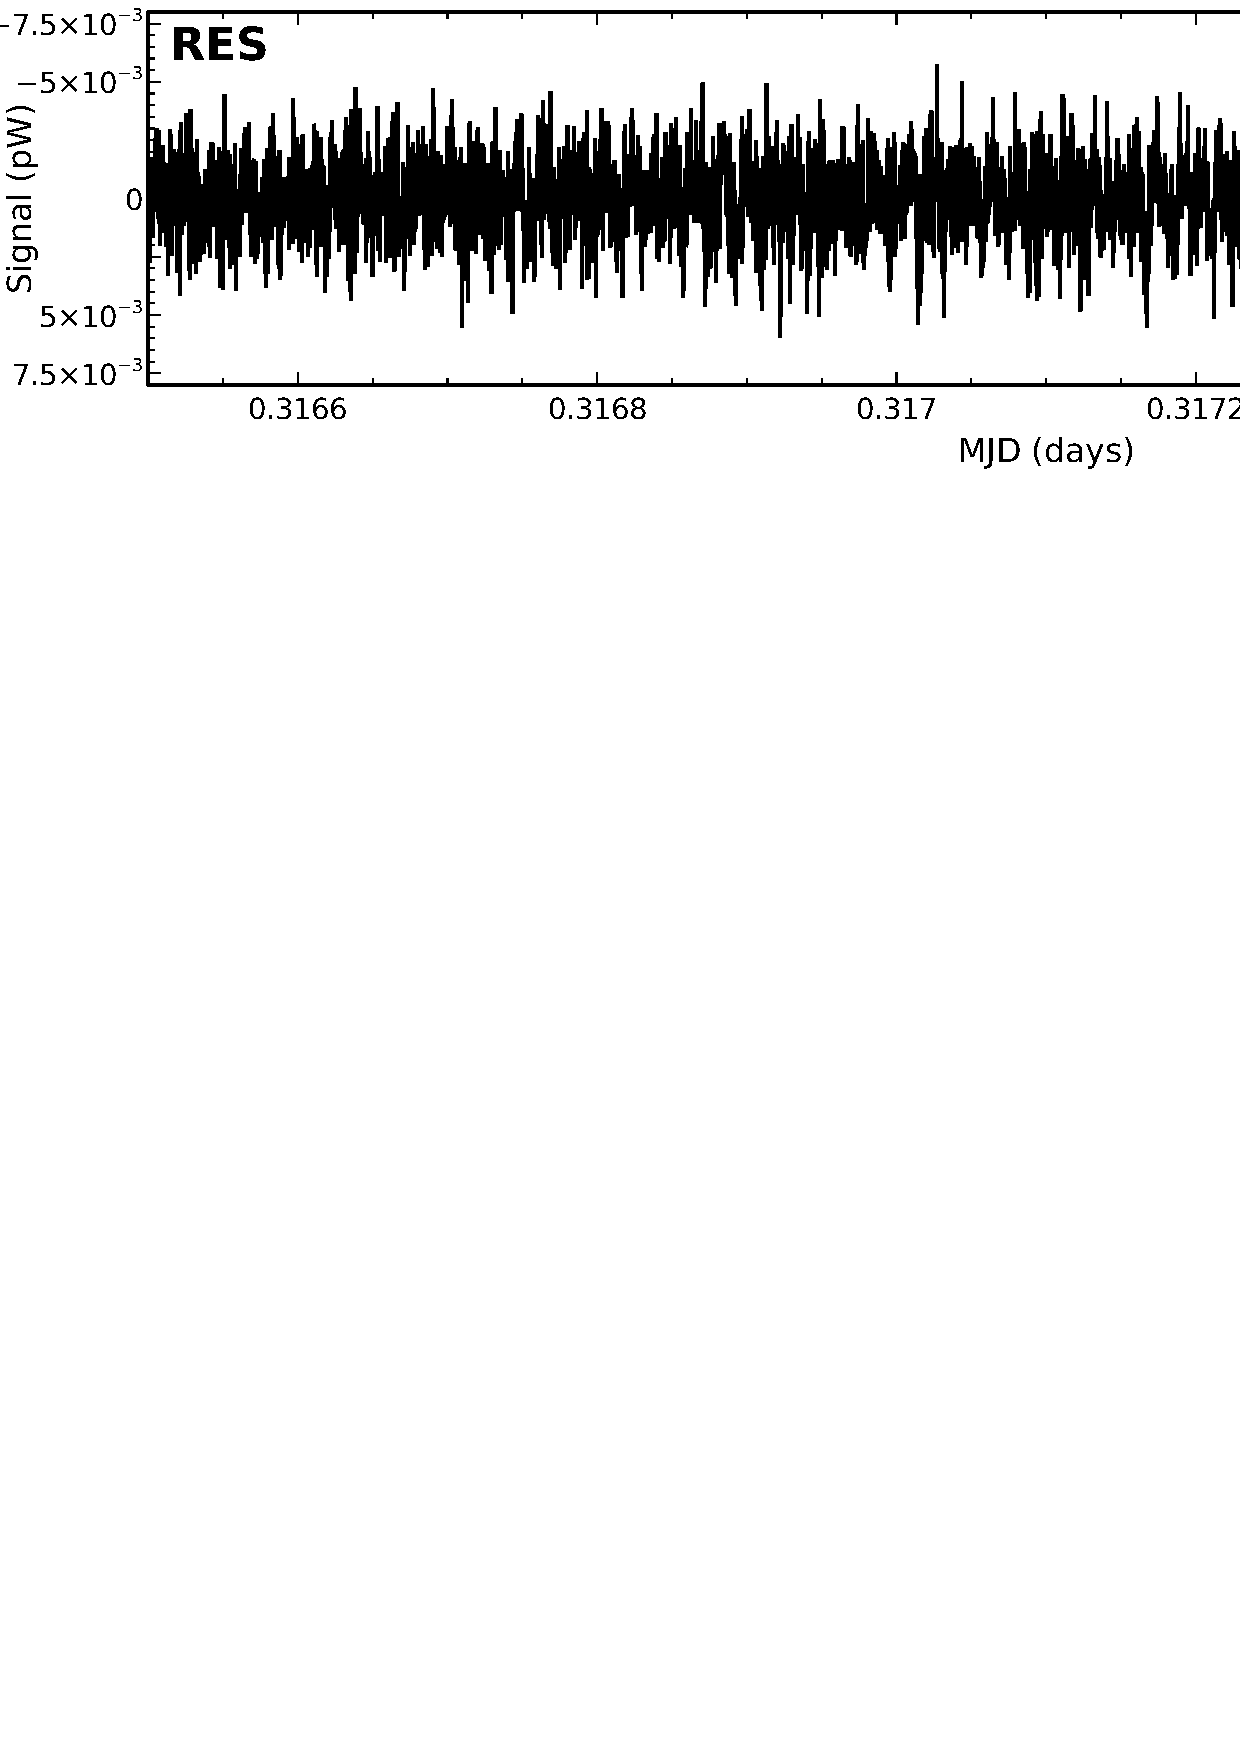
\includegraphics[width=\linewidth]{sc21_res} \\
\end{center}
\caption[Iterative models in the time domain]{\small These plots show
some of the models for a single bolometer, for part of an
observation of CRL~2688. From top to bottom: the \model{COM} model
containing signal common to all bolometers, the \model{FLT} model
containing residual low-frequency noise missed by \model{COM}, the
\model{AST} model with the astronomical signal showing as a positive
spike when this bolometer passes over the source, and the \model{RES}
model looking (as expected) like white noise.}
\label{fig:itercomp}
\end{figure}


\section{\xlabel{convergence}Stopping criteria}
\label{sec:converge}

The map-maker will stop processing either when the requested number of
iterations has been completed \textbf{OR} when the convergence
criterion specified in the configuration file is reached.


\textbf{Option 1: Fixed number of iterations}

Specifying the number of iterations in the configuration file is done
via the \xparam{NUMITER}{numiter} parameter. This is shown below for
\file{dimmconfig\_jsa\_generic.lis} (JSA stands for ``JCMT Science Archive'').

\begin{terminalv}
numiter = -25
\end{terminalv}

A positive value for \param{numiter} means that the requested number
of iterations will be executed. A negative value, as in the example
above, indicates that no more than this number of iterations should be
performed, \emph{but} that it may stop at fewer if convergence
(according to the noise criterion below) has been achieved.

\textbf{Option 2: Convergence parameter}

The convergence criterion is set by the \xparam{MAPTOL}{maptol} parameter.

When running the map-maker, \texttt{maptol} gives the average
normalised change in the value of map pixels
between subsequent iterations. Convergence is reached when the  mean
change across all pixels is less than the parameter \param{maptol}.
It has units of the noise in the map, thus \texttt{maptol}$=$0.05 means
a mean change in pixel value of $<$0.05\,$\sigma$. This option has the
advantage of directly assessing the noise in the resulting map.

The map-maker displays the normalised change in pixel values between
iterations at the end of each iteration. This value typically drops
rapidly to begin with and then flattens out, decreasing increasingly
slowly.  The printed values can be inspected to check convergence is
proceeding as expected. Be aware that setting \texttt{maptol} to much
lower than 0.05 will dramatically increase the length of time needed to
produce the final map, and may possibly result in convergence never being
achieved.

If you wish to perform further checks on the progress of convergence
while running the map-maker, you can use the \xparam{ITERMAP}{itermap}
option. This causes the map created by each iteration to be dumped to
disk for inspection (see \cref{Section}{sec:tweak}{Tweaking the
configuration file}).

\section{\xlabel{sec_masking}Masking}
\label{sec:masking}

The term \emph{masking} refers to the inclusion or exclusion of selected
bolometer samples from the estimate of specific models, based on the
positions of those samples within the output map. Masking can be applied
independently to the \model{AST}, \model{FLT} and \model{COM} models, as
described in the later sub-sections within this section.

A \emph{mask} is a selection of pixels within the output map. Normally
these pixels form one or more contiguous regions that enclose the areas
where significant sub-mm emission is expected (the ``source'' regions).
Pixels outside this mask are referred to as ``background pixels''. The use
to which such masks are put differs from model to model as described
later in model-specific sub-sections.

Masks fall into two broad categories:
\begin{itemize}

\item \textbf{dynamic masks} -- these are masks that change shape from one
iteration to the next.

\item \textbf{static masks} -- these are masks that retain the same shape
for all iterations.

\end{itemize}

Static masks are appropriate in cases where the areas containing significant
sub-mm emission are known in advance. If this is not the case, then the
mask needs to be based on evidence within the maps created at the end of
each iteration, resulting in the masks evolving from iteration to iteration
as the maps converge towards the final solution. Such \emph{dynamic} masks
have a potential problem  in that they can upset the convergence process by
introducing extra flexibility into the algorithm. For this reason, an
option is provided to freeze these masks after a fixed number of
iterations\footnote{Although by default masks are never frozen.}
(\emph{e.g.} see \xparam{AST.ZERO_FREEZE}{ast.zero\_freeze}) and this
is used within the specialist configuration file \fixconvergence\
described in \cref{Section}{sec:problem}{Configuration files for solving
specific problems}.

Each of the three models---\model{AST}, \model{FLT} and \model{COM}
---have an equivalent set of parameters to specify the masking (if any)
that should be used. Each set starts with the model name, followed by a
dot, followed by the parameter name. To enable masking, one or more of
these parameters needs to be set to a suitable value to define a mask, as
described below.

Static masks can be defined either as circles of specified radius,
centred on the source position (suitable for compact sources---see for
instance \xparam{AST.ZERO_CIRCLE}{ast.zero\_circle}), or by an external
image that uses special pixel values to indicate the source regions and
the background regions (suitable for extended sources---see for
instance \xparam{AST.ZERO_MASK}{ast.zero\_mask}). Within such ``external
masks'' all background pixels should be set to the Starlink \emph{bad} value
(see \xref{``Bad-pixel Masking''}{sun95}{se_badmasking} in SUN/95).
Pixels with any other value are treated as source pixels.
\cref{Section}{sec:maskbe}{Supplying an external mask} describes some
ways in which external masks can be generated.

Dynamic masks can be defined in several different ways:
\begin{enumerate}
\item By applying a simple threshold on the S/N ratio within the map
created at the end of each iteration (\emph{e.g.} see
\xparam{AST.ZERO_SNR}{ast.zero\_snr}).
\item By applying a simple threshold on the S/N ratio as above, and then
extending the resulting source regions down to a lower S/N value (\emph{e.g.}
see \xparam{AST.ZERO_SNRLO}{ast.zero\_snrlo}). This allows a low S/N
threshold to be used (which can sometimes help to avoid negative bowling
around the edges of extended sources) without introducing lots of isolated
pixels into the mask because of noise spikes in the map.
\item By applying a threshold on the number of bolometer samples falling
in each map pixel (\emph{e.g.} see \xparam{AST.ZERO_LOWHITS}
{ast.zero\_lowhits}). Because of the scanning strategy used with SCUBA-2
(see \cref{Section}{sec:mmodes}{Observing modes}), pixels near the edge of
the map will receive fewer bolometer samples than those near the centre,
and will therefore be noisier. Thus this scheme allows the noisy edges of
the map to be masked out. Whilst this is technically a dynamic mask---because
the number of samples falling in each pixel could potentially change
from iteration to iteration---in fact a mask based on hits per pixel
will usually only change very slightly from iteration to iteration.
\item By using an algorithm that automatically identifies features of a
given size in the map, similar to that used by the \textsc{Kappa}
\xref{\task{ffclean}}{sun95}{FFCLEAN} command (\emph{e.g.} see
\xparam{AST.ZERO_SNR_FFCLEAN}{ast.zero\_snr\_ffclean}). This can be a
useful alternative to simple S/N thresholding in cases where bright artificial
large-scale structures appear in the map. Such structures will result in
artificially large source regions in a simple S/N mask, which may in turn
cause the artificial structures to become even brighter and larger in
subsequent iterations. Using an \task{ffclean}-based mask instead will
restrict the mask to the brighter astronomical cores on top of such artificial
large-scale structures.
\end{enumerate}

Multiple masks can be used by selecting the appropriate configuration
parameters as described above. Whether the combined mask represents the
\emph{union} or \emph{intersection} of the individual masks is selected
using the parameters \xparam{AST.ZERO_UNION}{ast.zero\_union},
\xparam{FLT.ZERO_UNION}{flt.zero\_union} and \xparam{COM.ZERO_UNION}
{com.zero\_union}. By default, the union is used.



The masks used on the last iteration are stored in the \xref{\texttt{Quality}}
{sun95}{se_qualitymask} component of the NDF containing the output map.
A separate bit of the quality component is used for each model (\model{AST},
\model{FLT} or \model{COM}) that is being masked. These bits can be
viewed in various ways---see \cref{Section}{sec:maskshow}{Displaying masks}
and \cref{Section}{sec:itermaps}{Monitoring the map at the end of each
iteration}.

\begin{tip}
Be aware that the S/N ratio within individual map pixels depends on pixel
size---larger pixels will have higher S/N ratios than small pixels.
Therefore masks based on a specific S/N threshold will grow or shrink in
area as a function of pixel size. As a rough rule, if you double the pixel
size, you should also double the S/N thresholds to get a mask that covers a
similar area of the sky.
\end{tip}

\subsection{\xlabel{sec_astmask}AST masking}
\label{sec:astmask}
The iterative map-maker algorithm described earlier in this chapter
divides each cleaned bolometer value into four additive parts:
\begin{enumerate}
\item The common-mode signal (\model{COM}).
\item The low frequency background drift in each bolometer (\model{FLT}).
\item The astronomical signal (\model{AST}).
\item The left-over residual noise (\model{RES}).
\end{enumerate}

Whilst the value of each model is constrained to some extent by the
manner in which the model is calculated, there remains a large degree of
degeneracy in the algorithm. In other words, there are many different
ways in which each bolometer value can be divided up into the four values
listed above. For instance, any arbitrary change in the \model{AST} model
can be accommodated provided that equal and opposite changes are introduced
into the other model values so that the total value of all four components
remains the same.

The degeneracy between \model{COM} and \model{AST} is particularly
problematic, since it allows large scale features to appear in the map
(on the scale of the sub-array footprint) that are corrected for by equal
and opposite features in the \model{COM} model. Such features can appear
as gradients or ``saddles'' across the final map.

The purpose of masking the \model{AST} model is to apply an extra
constraint to the system to help break this degeneracy, and so avoid
these large-scale features. It functions by forcing the \model{AST} model
to zero at the end of each iteration for all samples that fall outside the
masked area on the sky (\emph{i.e.} samples that fall in the ``background''
areas of the map). Forcing the \model{AST} model to zero in this way means
that the \model{COM} model is more closely constrained.

Whilst this constraint is applied only in the background regions, its
effects are also felt part way into the source region because of the way in
which the \model{COM} model averages over a sub-array footprint. Thus source
regions that are much larger than a sub-array will still suffer from the
degeneracy between \model{COM} and \model{AST}, allowing arbitrary
large-scale background features to develop within the region, but these
features will become weaker as the edges of the mask are approached.

In order to avoid the final  map containing zero values in the background
region, it is necessary to avoid using \model{AST}-masking on the final
iteration. For this reason, by default one further iteration is
performed---without \model{AST}-masking---once the basic iterative algorithm has
converged (see \xparam{AST.ZERO_NOTLAST}{ast.zero\_notlast}).

All the configuration files supplied with \smurf\ use \model{AST}
masking, with the exception of \blankfield.

\subsection{\xlabel{sec_fltmask}FLT masking}
\label{sec:fltmask}

The \model{FLT} model estimates and removes a low frequency background
from each bolometer time-stream. To do this it uses an FFT-based high-pass
filter. Ringing around sudden transients---such as astronomical sources
--- is a natural consequence of all such filters, resulting in alternating
bright and dark rings around sources in the map. In most cases, the iterative
nature of the map-making algorithm eventually results in the rings
reducing to a much lower level, as more of the astronomical signal is removed
from the time stream on each iteration, causing the ring-inducing
transients to become weaker. However, this is not always completely
effective, and also slows down convergence.

For these reasons, it is often helpful to mask the \model{FLT} model.
This causes each bolometer time stream to be blanked out as the
bolometer passes over the source regions in the mask. Such blanked
sections are replaced by linear interpolation between the data on either
side of the blanked section. The effect of this is to remove the
transients that cause the ringing in the \model{FLT} model, and thus get
a better estimate of the low frequency background in each bolometer.

Such masking is most useful at the start of the iterative process,
before the bulk of the astronomical signal has been removed from the
time-streams. Indeed, if it is allowed to continue for too many iterations
it can cause its own problems that tend to slow down convergence. For
this reason, if \model{FLT} masking is used, it is (by default) limited
to two iterations---see \xparam{FLT.ZERO_NITER}{flt.zero\_niter}.

A difficulty with \model{FLT} masking is that the \model{FLT} model is
evaluated \emph{before} the map is made on each iteration. This means
that when the \model{FLT} model is evaluated on the first iteration,
there is no map available. This is not a problem if a static mask is
used, but if a dynamic mask is used, then it is not possible to calculate
the \model{FLT} mask on the first iteration (subsequent iterations will
create the mask on the basis of the map created at the end of the
previous iteration). This is a shame since \model{FLT} masking is most
beneficial on the first few iterations, whilst the bulk of the astronomical
signal is still present in the time streams. A scheme to get around this
problem is described in \cref{Section}{sec:skip}{Skipping the AST model}.

All the configuration files supplied with \smurf\ use \model{FLT}
masking, with the exception of \blankfield.

\subsection{\xlabel{sec_commask}COM masking}
\label{sec:commask}

The value of the \model{COM} model at a specific time-slice is the mean
of all remaining bolometer values at that time slice. If the \model{COM}
model is masked, bolometer samples that fall within the source regions
defined by the mask are excluded from this mean, thus removing the bias
introduced into the mean by bright astronomical sources. This results in
the \model{COM} model more accurately representing the varying common-mode
background value at each time slice. This can help to reduce negative
bowling around sources in the map, and can help to reduce the amount of
data that is rejected as being too poorly correlated with the common-mode
signal.

\model{COM} masking has the same difficulty as \model{FLT} masking in that
the \model{COM} model is evaluated \emph{before} the map is made on each
iteration, and so it is difficult to use dynamic masks with \model{COM}
masking. However, the solution described in \cref{Section}{sec:skip}{Skipping
the AST model} can be used for \model{COM} masking as for \model{FLT}
masking.

Currently, none of the configuration files supplied with \smurf\ use
\model{COM} masking.

\section{\xlabel{sec_skip}Skipping the AST model}
\label{sec:skip}
As discussed in \cref{Section}{sec:masking}{Masking}, \model{FLT}
masking is most effective on the early iterations (particularly the
first iteration). This is because the bulk of the astronomical signal is
still present in the time streams and is likely to cause bad ringing if
\model{FLT} masking is not used. However, since the \model{FLT} model
is evaluated before the map is made within each iteration, there is no map
available to use as the basis for a \model{FLT} mask on the very first
iteration.

One way to get round this is simply to use a static mask that does not
require a map to be available. However, this may not be possible,
particularly for extended sources where no \emph{a-priori} knowledge of the
source areas in the sub-mm may be available.

Another scheme is provided by the \xparam{AST.SKIP}{ast.skip}
configuration parameter. If \param{ast.skip} is set to a positive integer
$N$, the subtraction of the \model{AST} model from the time-series that
normally occurs at the end of each iteration is not performed on the
first $N$ iterations. This means that for the first $N$ iterations, the
time-series data remain unchanged, and consequently the models and the
resulting map are unchanged. Of itself, this does nothing useful---it
merely delays the first useful iteration. However, when combined with
\model{FLT} masking, it can be very beneficial because it allows a mask
to be created \emph{before} the first ``real'' iteration occurs
(\emph{i.e.} the first iteration that subtracts off the \model{AST}
model). This means that the first ``real'' map will have far less
ringing around bright sources than would otherwise be the case.  This in
turn means that far fewer iterations are required to correct this ringing.

It is also possible to use \param{ast.skip} with \model{COM} masking, but
the benefits are not so noticeable as for \model{FLT} masking.

The default value for \param{ast.skip} is zero, but the \brightextended\
and \jsageneric\ configuration files supplied with \smurf\ both set
\setparam{AST.SKIP}{ast.skip}{5} (and also use \model{FLT} masking).

\section{\xlabel{config}Specialised configuration files}
\label{sec:config}

Maps made by the pipeline using the
REDUCE\_SCAN recipe will use \file{dimmconfig\_jsa\_generic.lis} unless some
alternative configuration has been specified. This configuration file is
intended to provide a reasonably good map for all types of observations.
However, compromises have been made to reach that balance, the main one
being that some real extended structure is sacrificed in order to avoid
introducing artificial large scale structures.

Whilst \file{dimmconfig\_jsa\_generic.lis} is always a good place to start,
you will want to follow this up with a specialised configuration that will suit
your observation. A few specialised configuration files are supplied with
\smurf\ and can be found in \file{\$STARLINK\_DIR/share/smurf/}.

Note, any parameter for which no value is specified within the supplied
configuration will take on the default value listed in
\cref{Appendix}{app:parameters}{Configuration-parameter descriptions}.

Below is a description of each of the specialised configuration files.
The tables following each description list the parameters set by each file.
The files themselves are stored in \file{\$STARLINK\_DIR/share/smurf/}---they
are simple text files and so can be inspected easily.

\subsection{dimmconfig\_jsa\_generic.lis}
The \jsageneric\ configuration file is designed to handle all science data. This is a good
configuration file to start with if you are unsure how to proceed with your
data reduction.  You may notice that elements of this configuration are
common to the other specialised configuration files.

This configuration is optimised to suppress the creation of artificial
large scale structure within the final map. Consequently, some real
extended emission may be lost if this configuration is used. This goal is
achieved by:

\begin{enumerate}

\item Setting
\xparam{FLT.FILT_EDGE_LARGESCALE}{flt.filt\_edge\_largescale}) to 200
arcseconds so that the \model{FLT} model uses a  heavier than normal
filter.

\item Setting \xparam{COM.PERARRAY}{com.perarray} to 1, indicating that four separate
\model{COM} models should be used, one for each sub-array\footnote{By default, a single
\model{COM} model is used that represents the mean data value across all
four sub-arrays.}.

\item Using a mask to force the \model{AST} model to zero in the background regions
after each iteration (see parameters \xparam{AST.ZERO_SNR}{ast.zero\_snr}
and \xparam{AST.ZERO_SNRLO}{ast.zero\_snrlo}---also see
\cref{Section}{sec:astmask}{AST masking}).

\end{enumerate}

In addition the S/N threshold for DC steps (\xparam{DCTHRESH}{dcthresh})
is relaxed from 25 in the default file to 100 to avoid problems bright
sources triggering the step detection algorithm.

The other major feature of this configuration is that the subtraction of
the \model{AST} model is skipped on the first five iterations. In
conjunction with the use of \model{FLT} masking, this helps to speed up
convergence and minimise dark rings around bright source (see
\cref{Section}{sec:skip}{Skipping the AST model}.

\latex{\renewcommand*\arraystretch{1}}
\begin{table}[h!]
\centering
\begin{tabular}{|p{6.5cm}p{6.5cm}|}
\hline
\multicolumn{2}{|l|}{\file{dimmconfig\_jsa\_generic.lis}}\\
\hline
\setparam{AST.SKIP}{ast.skip}{5}              &\setparam{AST.ZERO_SNRLO}{ast.zero\_snrlo}{3}\\
\setparam{AST.ZERO_SNR}{ast.zero\_snr}{5}     &\setparam{COM.PERARRAY}{com.perarray}{1}\\
\setparam{DCTHRESH}{dcthresh}{100}            &\setparam{FLT.FILT_EDGE_LARGESCALE}{flt.filt\_edge\_largescale}{200}\\
\setparam{FLT.ZERO_SNRLO}{flt.zero\_snrlo}{3} &\setparam{FLT.ZERO_SNR}{flt.zero\_snr}{5}\\
\setparam{MAPTOL}{maptol}{0.01}               &\setparam{NUMITER}{numiter}{-25}\\
\setparam{NOISECLIPHIGH}{noisecliphigh}{10.0}\\
\hline
\end{tabular}
\end{table}




\subsection{dimmconfig\_blank\_field.lis}

The \blankfield\ configuration is tuned for blank field surveys for which the goal
is to detect extremely low signal-to-noise point sources within otherwise
blank fields.

Applying a high-pass filter (\model{FLT}) on each iteration can result in
convergence problems when there is little or no signal in the
map. Instead, a single, harsher high-pass filter is applied as a
pre-processing step (corresponding to 200-arcsec scales at both
450\,$\mu$m and 850\,$\mu$m). There are also more conservative cuts to
remove noisy/problematic bolometers. Only 4 (positive) iterations are
requested as there is no signal to confuse to models.

The option \xparam{COM.PERARRAY}{com.perarray}~=~1 requires the \model{COM} model to
be fit to each sub-array independently. This improves the overall fit
but with the loss of any structure on scales larger than a single
sub-array---not an issue for blank fields.

\cref{Figure}{fig:bfcompare}{The images below} shows the sharp
contrast in the output map between reducing data with the default
configuration file and using \file{dimmconfig\_blank\_field.lis}.

Blank-field maps commonly have a matched filter applied as part of the
post-processing to aid source detection (see
\cref{Section}{sec:mf}{Point-source detection}), however this is not
applied by the map-maker.

\begin{figure}[t!]
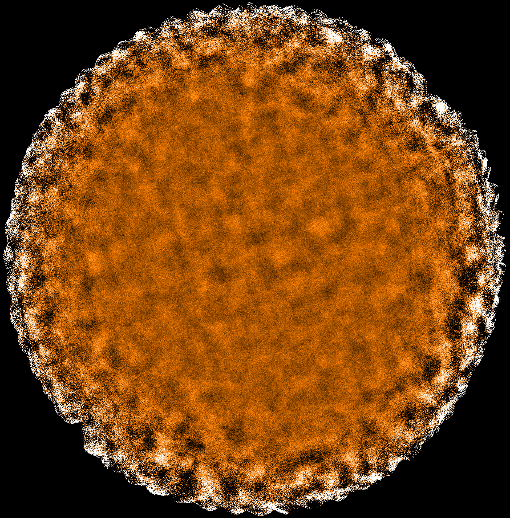
\includegraphics[width=0.47\linewidth]{sc21_cosmo1-def}
\hspace{3mm}
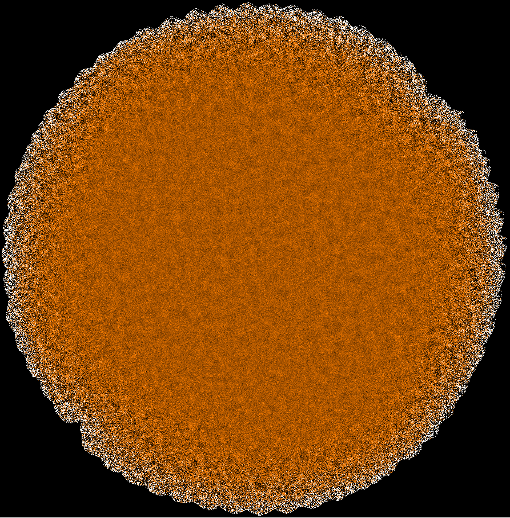
\includegraphics[width=0.47\linewidth]{sc21_cosmo1-bf}
\caption[Example map reduced with \file{dimmconfig\_blank\_field.lis}]{
    Maps of a deep cosmology field reduced with \textbf{(left)}
    default parameter values (\emph{i.e.} no configuration file) and
    \textbf{(right)} \file{dimmconfig\_blank\_field.lis} \label{fig:bfcompare}}.
\end{figure}



% The tildes around the equal sign are to ensure HTML table field is
% not wrapped after the parameter name.
\renewcommand*\arraystretch{0.95}
\begin{table}[h!]
\centering
\begin{tabular}{|p{6.5cm}p{7.0cm}|}
\hline
\multicolumn{2}{|l|}{\file{dimmconfig\_blank\_field.lis}}\\
\hline
\setparam{NUMITER}{numiter}{4}           & \setparam{FILT_EDGE_LARGESCALE}{flt\_edge\_largescale}{200}\\
\setparam{SPIKETHRESH}{spikethresh}{10}  & \setparam{MODELORDER}{modelorder}{(com,ext,ast,noi)}\\
\setparam{COM.PERARRAY}{com.perarray}{1} &\\
\hline
\end{tabular}
\end{table}




\subsection{dimmconfig\_bright\_compact.lis}
\label{sec:brightcompact}

The \brightcompact\ configuration should be used for producing maps of
bright, isolated compact sources that are positioned at the centre of the
map (\emph{e.g.} calibrators).

The addition of the \xparam{AST.ZERO_CIRCLE}{ast.zero\_circle} parameter
is used to constrain the map to zero beyond a radius of 1\,arc-min from
the source centre (see \cref{Section}{sec:astmask}{AST masking}).  This
strategy helps with map convergence significantly, and can provide good
maps of bright sources, even in cases where scan patterns failed to
complete in full.

\xparam{COM.PERARRAY}{com.perarray} is set to 1 indicating that a \model{COM} model
should be fit separately for each sub-array. This is not advised for
extended sources as signal on scales larger than a single sub-array is
lost, but is fine for a compact central source. Likewise, the filtering
is tighter. The S/N threshold for DC steps (\xparam{DCTHRESH}{dcthresh}) is relaxed from
25 in the default file to 100 to avoid problems associated with bright sources.

The values of the parameters controlling the \model{COM} model are
modified to relax the test that compares each bolometer to the common
mode. This is because the algorithm that compares each bolometer to the
common-mode can be fooled by a bright compact source passing across
individual bolometers. Likewise the test for DC steps within each
bolometer baseline is also relaxed (parameter \xparam{DCTHRESH}{dcthresh}).

% The tildes around the equal sign are to ensure HTML table field is
% not wrapped after the parameter name.
\latex{\renewcommand*\arraystretch{0.95}}
\begin{table}[h!]
\centering
\begin{tabular}{|p{6.5cm}p{7.0cm}|}
\hline
\multicolumn{2}{|l|}{\file{dimmconfig\_bright\_compact.lis}}\\
\hline
\setparam{NUMITER}{numiter}{-40}                & \setparam{FLT.FILT_EDGE_LARGESCALE}{flt.filt\_edge\_largescale}{200}\\
\setparam{COM.PERARRAY}{com.perarray}{1}        & \setparam{FLT.ZERO_CIRCLE}{flt.zero\_circle}{(0.016666)}\\
\setparam{AST.ZERO_CIRCLE}{ast.zero\_circle}{(0.0166666666)}&\\
\setparam{NOISECLIPHIGH}{noisecliphigh}{10.0}   & \setparam{DCTHRESH}{dcthresh}{100}\\
\setparam{COM.CORR_TOL}{com.corr\_tol}{7}       & \setparam{COM.GAIN_TOL}{com.gain\_tol}{7}\\
\setparam{COM.GAIN_ABSTOL}{com.gain\_abstol}{5} & \\
\hline
\end{tabular}
\end{table}


\subsection{dimmconfig\_bright\_extended.lis}

\begin{figure}[t!]
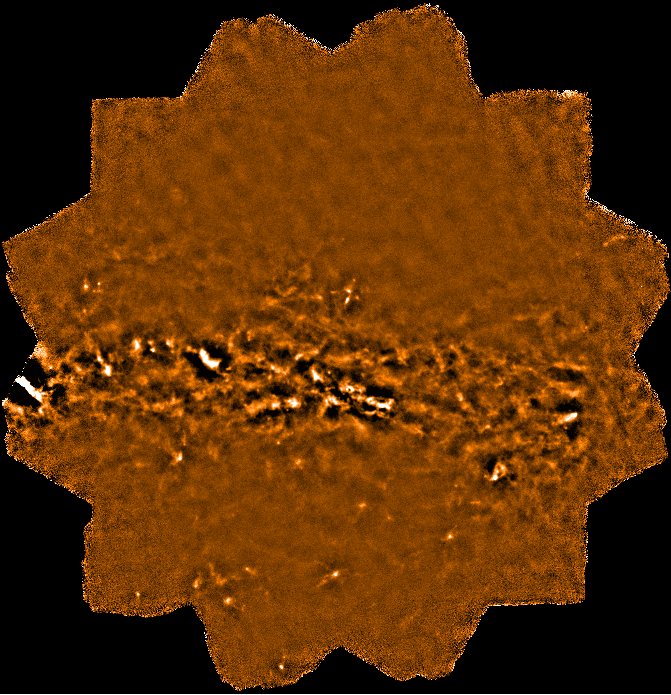
\includegraphics[width=0.47\linewidth]{sc21_gal_def}
\hspace{3mm}
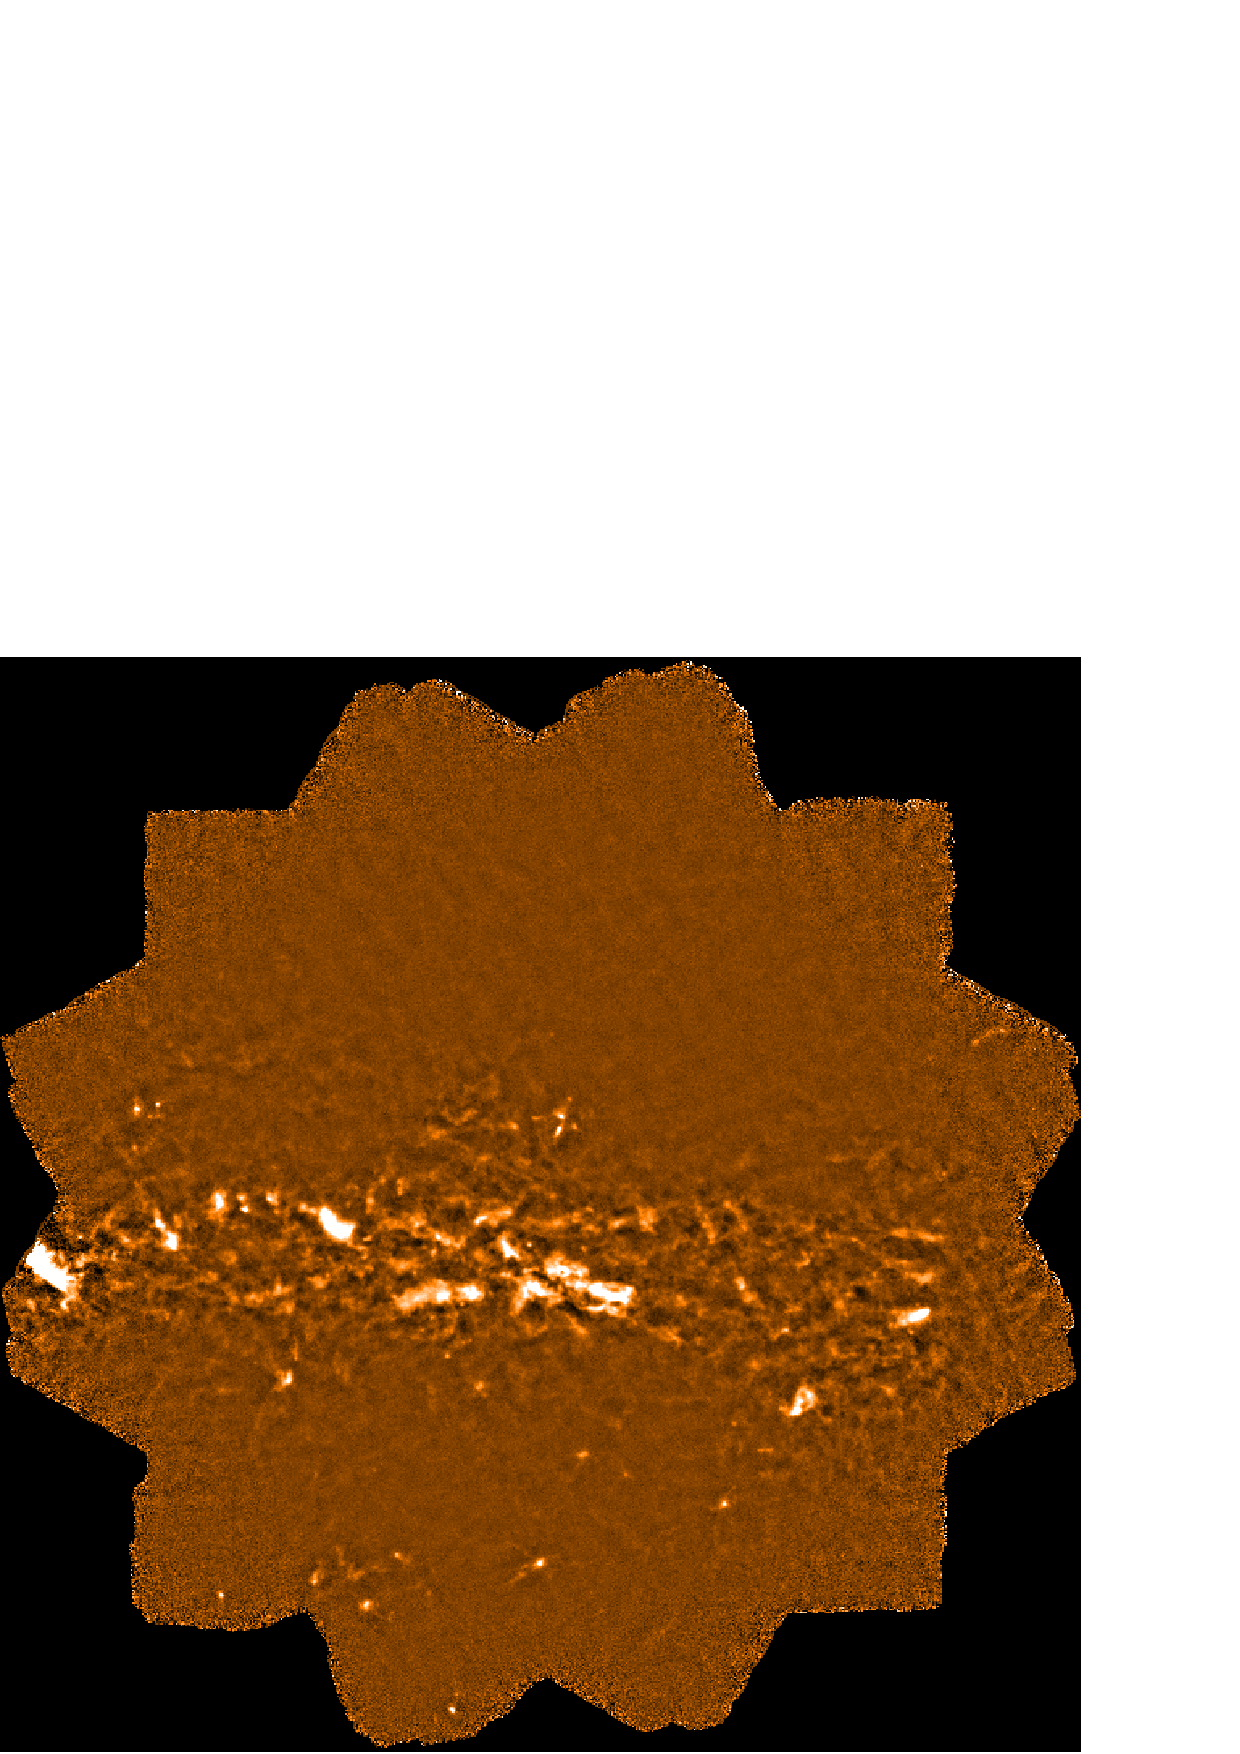
\includegraphics[width=0.47\linewidth]{sc21_gal_brex}
\caption[Example map reduced with
  \file{dimmconfig\_bright\_extended.lis}]
   {A region towards the Galactic Centre reduced with \textbf{(left)}
   default parameter values (\emph{i.e.} no configuration file) \textbf{(right)}
   \file{dimmconfig\_bright\_extended.lis}.\label{fig:becompare}}
\end{figure}

The \brightextended\ configuration is for reducing maps that contain
emission that is extended to some degree and contains some bright
regions. Here, the combination of \xparam{AST.ZERO_SNR}{ast.zero\_snr}
and \xparam{AST.ZERO_SNRLO}{ast.zero\_snrlo} is used to identify components of
the \model{AST} model wherever the S/N is higher than 3$\sigma$ and then
to expand this basic mask down to an SNR equal to 2$\sigma$ without introducing
any new isolated source areas (see \cref{Section}{sec:astmask}{AST masking}).
\xparam{NUMITER}{numiter} has been raised to \texttt{-40}, as more iterations are
required to maximise the sensitivity to large dynamic signal ranges in the map.

The other major feature of this configuration is that the subtraction of
the \model{AST} model is skipped on the first five iterations. In
conjunction with the use of \model{FLT} masking, this helps to speed up
convergence and minimise dark bowls around bright source (see
\cref{Section}{sec:skip}{Skipping the AST model}.

\cref{Figure}{fig:becompare}{The images below} shows a comparison
between maps reduced with the default configuration file and using
\file{dimmconfig\_bright\_extended.lis}; the most noticeable
difference is the improvement in the bowling around strong sources.

\latex{\renewcommand*\arraystretch{1}}
\begin{table}[h!]
\centering
\begin{tabular}{|p{6.5cm}p{6.5cm}|}
\hline
\multicolumn{2}{|l|}{\file{dimmconfig\_bright\_extended.lis}}\\
\hline
\setparam{NUMITER}{numiter}{-40}              & \setparam{FLT.FILT_EDGE_LARGESCALE}{flt.filt\_edge\_largescale}{480}\\
\setparam{AST.ZERO_SNR}{ast.zero\_snr}{3}     & \setparam{AST.ZERO_SNRLO}{ast.zero\_snrlo}{2}\\
\setparam{AST.SKIP}{ast.skip}{5}              & \setparam{FLT.ZERO_SNR}{flt.zero\_snr}{5}\\
\setparam{FLT.ZERO_SNRLO}{flt.zero\_snrlo}{3} & \\
\hline
\end{tabular}
\end{table}

\subsection{dimmconfig\_pca.lis}

The newest dimmconfig file (2019) is called: dimmconfig\_pca.lis.  This parameter file can be combined with
other dimmconfig files to tell makemap to include a Principal Component Analysis (PCA) model in its iterative algorithm
(the PCA model removes noise signals that are correlated between multiple bolometer time-streams).
For instance, to use a PCA model when creating a map of a bright extended source, you could run makemap as follows:

\begin{terminalv}
% more conf
^$STARLINK_DIR/share/smurf/dimmconfig_bright_extended.lis
^$STARLINK_DIR/share/smurf/dimmconfig_pca.lis
% makemap config=^conf
\end{terminalv}

To process compact sources, change “bright\_extended” above to “bright\_compact“.

\begin{figure}
\includegraphics[width=0.9\linewidth]{sc21_BrightExtendedPCA.png}\\
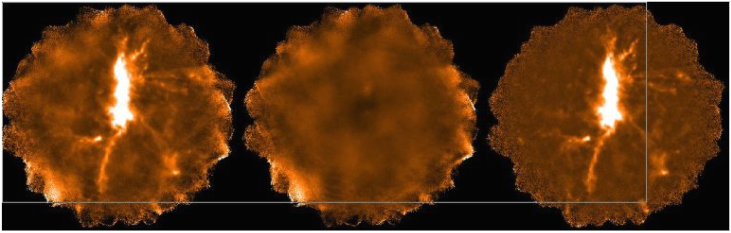
\includegraphics[width=0.9\linewidth]{sc21_PCADifference.png}
\caption[PCA dimmconfig results]
   {\textit{Top}: Four 850-$\mu$m maps made with the basic ``bright extended'' dimmconfig. \textit{Middle}: The results of adding in the new PCA dimmconfig file. \textit{Bottom}: The mosaics of the top and middle rows (left and right, respectively) with a difference map in between.}
   \label{fig:PCAfig}
\end{figure}

Using a PCA model can help to reduce the spurious extended structures
that often appear in SCUBA-2 maps (although this benefit is bought at
the cost of a much extended run time). For instance, four 850-$\mu$m
maps of DR~21 are presented in \cref{Figure}{fig:PCAfig}{}.  Its top
row shows the maps made with the basic ``bright extendedd''
dimmconfig, the middle row shows the results of adding in the new PCA
dimmconfig, and the bottom row shows mosaics of the top and middle
rows (left and right, respectively) with a difference map in between.

\section{\xlabel{problem}Configuration files for solving specific problems}
\label{sec:problem}

Two additional configuration files are available that can be used to supplement your
configuration file in order to solve specific problems:

\begin{itemize}[noitemsep]

\item \fixconvergence\ to help your map converge. It does this by preventing masks
from changing, and by freezing the flags that identify aberrant bolometers. Both of
these restrictions are imposed only after 10 iterations have been performed.

\item \fixblobs\ to remove large ``blooms'' or smooth blobs of spurious emission
in your map. These can be caused by ringing induced by unidentified steps or
spikes in the bolometer time-streams. The fix is to look for oscillations
within the time-streams following the \model{FLT} model, and flag such
time-slices as unusable.  In addition, time slices at which the four sub-arrays
see significantly different common-mode values are also flagged as unusable.

\end{itemize}

These files provide a few additional settings that should be added to
some other configuration in order to achieve the desired fix. For
instance, a configuration file containing the following two lines would
indicate that values from both \file{dimmconfig\_bright\_extended.lis} and
\file{dimmconfig\_fix\_blobs.lis} should be used:

\begin{terminalv}
^/star/share/smurf/dimmconfig_bright_extended.lis
^/star/share/smurf/dimmconfig_fix_blobs.lis
\end{terminalv}

This reads a set of configuration parameter from the
\file{dimmconfig\_bright\_extended.lis} file, and then assigns new values for just
those parameters defined in \file{dimmconfig\_fix\_blobs.lis}. These values override
the values specified in \file{dimmconfig\_bright\_extended.lis}.

The parameters in these files are discussed further
\cref{Chapter}{sec:tweak}{Tailoring Your Reduction}.



